\documentclass[11pt,a4paper]{article}
\usepackage[T2A]{fontenc}
\usepackage[utf8]{inputenc}
\usepackage[russian]{babel}
\usepackage[margin=2.2cm]{geometry}
\usepackage{amsmath,amssymb}
\usepackage{booktabs}
\usepackage{graphicx}
\newcommand{\code}[1]{\texttt{#1}}

\title{Функции выживания со сдвигом на время перехода\\\large расчёт свёрткой на сетке в \code{survpm}}
\date{26 октября 2026}

\begin{document}
\maketitle

\section{Что есть сейчас}

\paragraph{Модель.} Сеть состояний с одним токеном. Из состояния $s$ выход $s\to d$
выбирается с вероятностью $p_{sd}$, затем токен ждёт в $s$ время
$\Delta t\sim f_{sd}$ (CDF $G_{sd}$, $S_{sd}=1-G_{sd}$), отсчитанное от момента прихода в $s$.
Параметры $p_{sd}$ и $f_{sd}$ оцениваются совместной MLE с цензурой (\code{estimate\_network}).

\paragraph{Время процесса.} Нас интересует $T$~--- время от входа в начальное состояние
(Registration) до конечного (Discharge), и $S(t)=P(T>t)$. Это сумма $\Delta t$ по
случайному пути, поэтому каждое следующее ожидание начинается со сдвигом на момент прихода
в своё состояние.

\paragraph{Как считается сейчас.} \code{CensoredStateNet.survival()} делает это
Монте-Карло: \code{simulate()} прогоняет $n=10\,000$ трасс, на каждом шаге выбирает выход по
$p_{sd}$ и прибавляет $\Delta t$, случайно сгенерированное из $f_{sd}$. Затем
\[
\hat S(t)=1-\frac{\#\{i:\ T_i\le t\}}{n},
\]
где $T_i=\infty$, если трасса до Discharge не дошла. Кривая ступенчатая, шумит
(максимальное отклонение от эталона около $0.013$, табл.~\ref{tab:check}) и зависит от \code{seed}.
Кривые <<из промежуточного состояния>> и прогноз для незавершённого случая не считаются.

\section{Что предлагается}

\subsection{Уравнение со сдвигом}

Для каждого состояния $s$ введём
\[
F_s(t)=P\bigl(\text{пришедший в $s$ в момент 0 токен дойдёт до Discharge к $t$}\bigr),
\quad S_s=1-F_s.
\]
Если первый переход из $s$ произошёл в момент $u$ в состояние $d$, то на оставшийся путь
осталось $t-u$. Усредняя по выбору выхода и по $u$:
\begin{equation}\label{eq:renewal}
F_s(t)=\sum_d p_{sd}\int_0^t f_{sd}(u)\,F_d(t-u)\,du,\qquad
F_{\text{Discharge}}\equiv 1,\qquad F_s\equiv 0\ \text{для тупиков}.
\end{equation}
Функция следующего состояния $F_d$ берётся со сдвигом на $u$~--- момент прихода в $d$.
Это уравнение марковского восстановления для полумарковского процесса; порядок <<сначала выбор,
потом время>> тот же, что в правдоподобии, по которому оценена модель.
Искомая кривая $S(t)=1-F_{\text{Registration}}(t)$, а остальные $F_s$ получаются попутно.

\paragraph{Пример.} Для цепочки $A\to B\to D$: $F_B=G_{BD}$ и
$F_A(t)=\int_0^t f_{AB}(u)\,G_{BD}(t-u)\,du$, то есть обычная свёртка двух времён.
В сети с ветвлениями и циклами явной формулы нет, поэтому~\eqref{eq:renewal} решается на сетке.

\subsection{Расчёт на сетке}

Возьмём шаг $h$ и округлим время каждого перехода до ближайшего узла $jh$. Масса узла
\[
g_{sd}[0]=G_{sd}(h/2),\qquad g_{sd}[j]=G_{sd}\bigl((j+\tfrac12)h\bigr)-G_{sd}\bigl((j-\tfrac12)h\bigr),\ j\ge1.
\]
Интеграл в~\eqref{eq:renewal} превращается в сумму
\[
F_s[k]=\sum_d p_{sd}\,g_{sd}[0]\,F_d[k]\;+\;\underbrace{\sum_d p_{sd}\sum_{j=1}^{k}g_{sd}[j]\,F_d[k-j]}_{b_s[k]}.
\]
Второе слагаемое $b_s[k]$ зависит только от уже посчитанных $F[0..k-1]$. Первое описывает
переходы короче полушага (в Sepsis их много: часть переходов длится минуты); они связывают
состояния в один момент, поэтому для всех нетерминальных состояний сразу решается система
\[
(I-P_0)\,F[k]=b[k]+P_0^{\to\text{Discharge}},\qquad (P_0)_{sd}=p_{sd}\,g_{sd}[0].
\]
Матрица $I-P_0$ одна для всех $k$ и обращается один раз. Так счёт идёт вперёд по
$k=0,1,2,\dots$, и циклы (возвраты в состояние) ему не мешают.

\paragraph{Полшага.} После округления событие <<время $\le kh$>> соответствует истинному
<<времени $\le (k+\frac12)h$>>, поэтому $F[k]$ относится к моменту $(k+\frac12)h$. С этим сдвигом
ошибка убывает как $O(h^2)$: на цепочке $\mathrm{Exp}(1)\to\mathrm{Exp}(1)$ она $1.2\cdot10^{-3}$
при $h=0.1$ и $1.2\cdot10^{-5}$ при $h=0.01$ (без сдвига было бы $1.9\cdot10^{-2}$ и $1.8\cdot10^{-3}$).

\paragraph{Цена.} $O(E\,K^2)$ операций, $E$~--- число рёбер, $K=\lceil\text{горизонт}/h\rceil$.
Масса за горизонтом просто не учитывается, поэтому горизонт должен покрывать интересующие $t$.

\subsection{Прогноз для идущего случая}

Пусть токен уже $a$ дней находится в $s$. Тогда выходы, которые <<должны были>> сработать раньше,
становятся менее вероятны, а ожидание~--- условным:
\[
p_{sd}(a)=\frac{p_{sd}\,S_{sd}(a)}{\sum_{d'}p_{sd'}\,S_{sd'}(a)},\qquad
f_{sd}(u\mid a)=\frac{f_{sd}(a+u)}{S_{sd}(a)},
\]
\[
F(t\mid s,a)=\sum_d p_{sd}(a)\int_0^t f_{sd}(u\mid a)\,F_d(t-u)\,du .
\]
Здесь $t$ отсчитывается от текущего момента, а $F_d$ берутся из уже посчитанной сетки, так что
нужна лишь одна свёртка на каждый выход. Если с начала процесса прошло $\tau$, то
в абсолютном времени $S(t\mid\tau)=S(t-\tau\mid s,a)$. Для экспонент $F(t\mid s,a)=F_s(t)$
(отсутствие памяти), это проверяется в тестах.

\subsection{Роль цензуры}

Цензура входит только в оценку $p_{sd}$ и $f_{sd}$. Кривые~\eqref{eq:renewal} описывают процесс
без потери наблюдения, как и симуляция с \code{censoring=False}. С данными их сравнивают через
Каплана--Майера (метрики \code{km\_sup}, \code{ibs} в \code{survpm.metrics}).

\section{Реализация}

Новый модуль \code{survpm/curves.py} (ядро, только numpy/scipy) и методы модели:
\begin{center}\small
\begin{tabular}{@{}lp{5.2cm}@{}}
\toprule
\code{model.survival(t, method='grid', step=None)} & $S(t)$ свёрткой; по умолчанию $h=\max t/2000$\\
\code{model.state\_curves(horizon, step=None)} & таблица $S_s(t)$ для всех состояний\\
\code{model.residual\_survival(s, a, t)} & $S(t\mid s,a)$ для идущего случая\\
\code{curves.completion\_cdf(edges, terminal, horizon, step)} & матрица $F_s[k]$\\
\bottomrule
\end{tabular}
\end{center}
По умолчанию \code{survival()} по-прежнему симулирует (\code{method='sim'}), поэтому ноутбуки и
метрики дают те же числа. Генерация трасс и оценка не менялись.

\section{Проверка}

Эталон~--- симуляция на $200\,000$ трасс; её собственный шум по супремуму порядка $0.002$--$0.003$,
поэтому меньшие расхождения уже не различимы.

\begin{table}[h]
\centering
\caption{$\sup_t|S(t)-S_{\text{эталон}}(t)|$ и время счёта}\label{tab:check}
\begin{tabular}{lcccc}
\toprule
& \multicolumn{2}{c}{симуляция, $n=10^4$} & \multicolumn{2}{c}{сетка} \\
\cmidrule(lr){2-3}\cmidrule(lr){4-5}
сеть & отклонение & сек & отклонение & сек \\
\midrule
A--D, истинная ($h=0.05$) & 0.011 & 1.35 & 0.0009 & 0.06 \\
A--D, оценённая ($h=0.05$) & 0.014 & 1.05 & 0.0014 & 0.05 \\
Sepsis, 12 рёбер ($h=0.5$) & 0.013 & 2.43 & 0.012 & 0.005 \\
Sepsis ($h=0.1$) & & & 0.0038 & 0.03 \\
Sepsis ($h=0.02$) & & & 0.0016 & 0.35 \\
\bottomrule
\end{tabular}
\end{table}

На Sepsis грубый шаг $h=0.5$ дня даёт заметную ошибку: многие переходы короче шага.
Шаг порядка 0.02--0.1 дня (полчаса--2 часа) даёт точность выше симуляции и считается
быстрее неё. Прогноз остатка (состояние B сети A--D, $a=0,2,8$ дней) совпадает с
Монте-Карло на $40\,000$ трасс с отклонением $\le0.005$ (рис.~\ref{fig:residual}).

\begin{figure}[h]
\centering
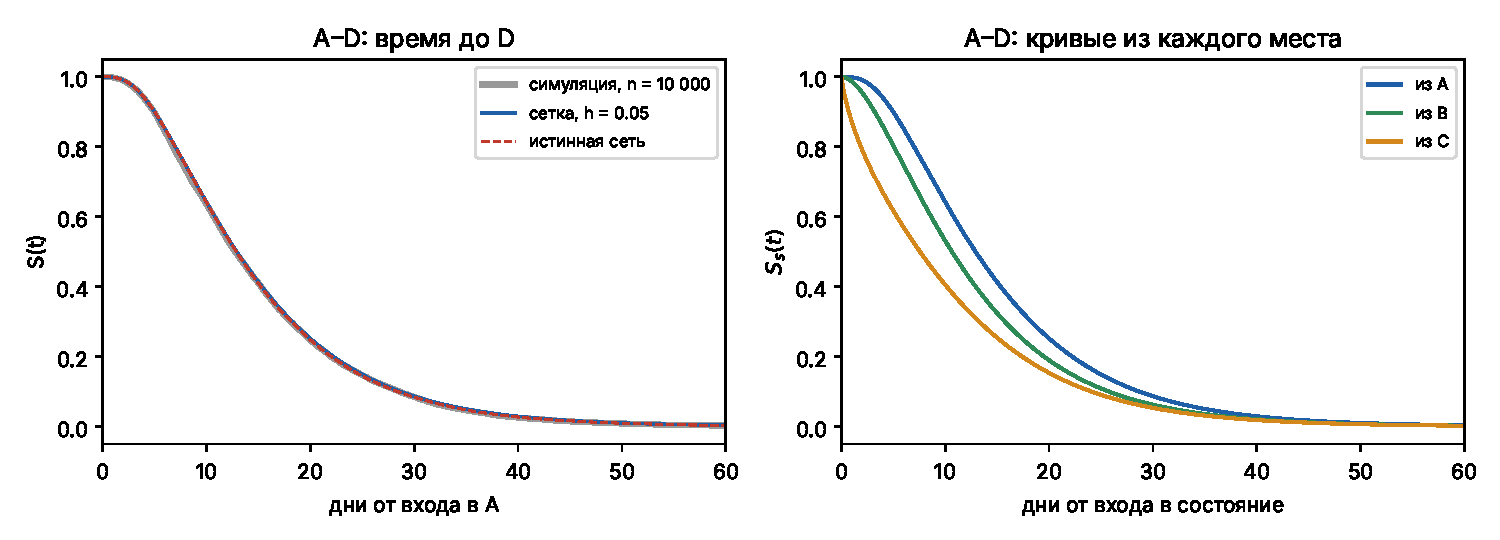
\includegraphics[width=\linewidth]{figures/survival_grid_ad.pdf}
\caption{A--D. Слева: сетка совпадает с симуляцией и близка к истинной сети.
Справа: кривые $S_s(t)$ из каждого состояния.}
\end{figure}

\begin{figure}[h]
\centering
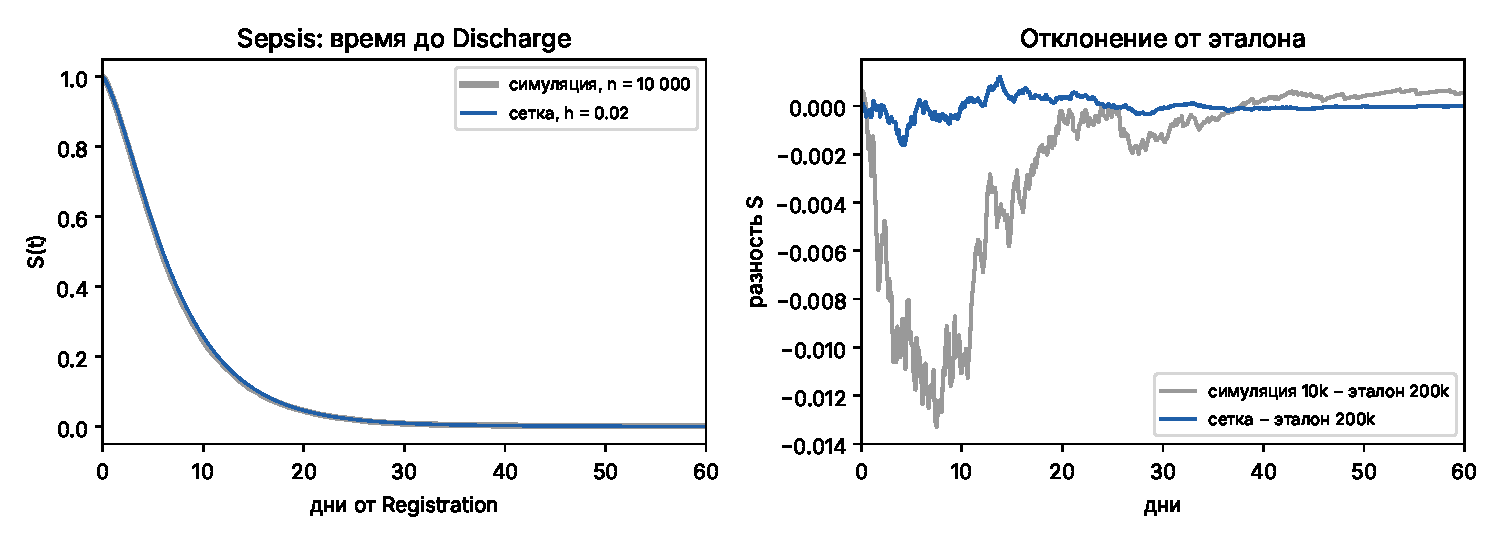
\includegraphics[width=\linewidth]{figures/survival_grid_sepsis.pdf}
\caption{Sepsis. Справа: отклонение от эталона $200\,000$ трасс; у сетки нет шума.}
\end{figure}

\begin{figure}[h]
\centering
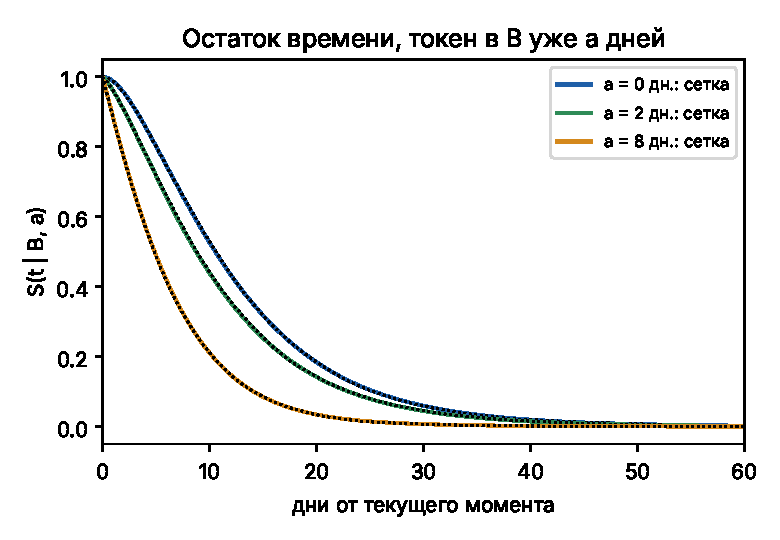
\includegraphics[width=.6\linewidth]{figures/survival_grid_residual.pdf}
\caption{Остаток времени до D, если токен уже $a$ дней в B: сетка (цвет) и Монте-Карло (пунктир).}
\label{fig:residual}
\end{figure}

\section{Ограничения и дальше}

\begin{itemize}
\item Модель полумарковская: время ожидания зависит только от текущего состояния и времени
с момента прихода в него, но не от истории пути. Это то же допущение, что и в оценке.
\item Шаг $h$ надо выбирать меньше характерных коротких переходов; на Sepsis~--- не больше
$0.1$ дня.
\item Можно перевести метрики \code{km\_sup}, \code{km\_l1\_days}, \code{ibs} на
\code{method='grid'}: результаты станут без шума и не будут зависеть от \code{seed}.
Пока это не сделано, чтобы не менять уже посчитанные таблицы.
\end{itemize}

\end{document}
